\documentclass[]{elsarticle} %review=doublespace preprint=single 5p=2 column
%%% Begin My package additions %%%%%%%%%%%%%%%%%%%
\usepackage[hyphens]{url}

  \journal{Journal of Memory and Language} % Sets Journal name


\usepackage{lineno} % add
\providecommand{\tightlist}{%
  \setlength{\itemsep}{0pt}\setlength{\parskip}{0pt}}

\usepackage{graphicx}
%%%%%%%%%%%%%%%% end my additions to header

\usepackage[T1]{fontenc}
\usepackage{lmodern}
\usepackage{amssymb,amsmath}
\usepackage{ifxetex,ifluatex}
\usepackage{fixltx2e} % provides \textsubscript
% use upquote if available, for straight quotes in verbatim environments
\IfFileExists{upquote.sty}{\usepackage{upquote}}{}
\ifnum 0\ifxetex 1\fi\ifluatex 1\fi=0 % if pdftex
  \usepackage[utf8]{inputenc}
\else % if luatex or xelatex
  \usepackage{fontspec}
  \ifxetex
    \usepackage{xltxtra,xunicode}
  \fi
  \defaultfontfeatures{Mapping=tex-text,Scale=MatchLowercase}
  \newcommand{\euro}{€}
\fi
% use microtype if available
\IfFileExists{microtype.sty}{\usepackage{microtype}}{}
\bibliographystyle{elsarticle-harv}
\usepackage{graphicx}
\ifxetex
  \usepackage[setpagesize=false, % page size defined by xetex
              unicode=false, % unicode breaks when used with xetex
              xetex]{hyperref}
\else
  \usepackage[unicode=true]{hyperref}
\fi
\hypersetup{breaklinks=true,
            bookmarks=true,
            pdfauthor={},
            pdftitle={Assessing replication rates in journals of experimental linguistics},
            colorlinks=false,
            urlcolor=blue,
            linkcolor=magenta,
            pdfborder={0 0 0}}
\urlstyle{same}  % don't use monospace font for urls

\setcounter{secnumdepth}{0}
% Pandoc toggle for numbering sections (defaults to be off)
\setcounter{secnumdepth}{0}

% Pandoc citation processing
\newlength{\cslhangindent}
\setlength{\cslhangindent}{1.5em}
\newlength{\csllabelwidth}
\setlength{\csllabelwidth}{3em}
% for Pandoc 2.8 to 2.10.1
\newenvironment{cslreferences}%
  {}%
  {\par}
% For Pandoc 2.11+
\newenvironment{CSLReferences}[2] % #1 hanging-ident, #2 entry spacing
 {% don't indent paragraphs
  \setlength{\parindent}{0pt}
  % turn on hanging indent if param 1 is 1
  \ifodd #1 \everypar{\setlength{\hangindent}{\cslhangindent}}\ignorespaces\fi
  % set entry spacing
  \ifnum #2 > 0
  \setlength{\parskip}{#2\baselineskip}
  \fi
 }%
 {}
\usepackage{calc}
\newcommand{\CSLBlock}[1]{#1\hfill\break}
\newcommand{\CSLLeftMargin}[1]{\parbox[t]{\csllabelwidth}{#1}}
\newcommand{\CSLRightInline}[1]{\parbox[t]{\linewidth - \csllabelwidth}{#1}\break}
\newcommand{\CSLIndent}[1]{\hspace{\cslhangindent}#1}

% Pandoc header



\begin{document}
\begin{frontmatter}

  \title{Assessing replication rates in journals of experimental
linguistics}
    \author[University of Osnabrück]{Kristina Kobrock\corref{1}}
   \ead{kkobrock@uni-osnabrueck.de} 
    \author[University of Oslo]{Timo B. Roettger}
  
      \address[University of Osnabrück]{Department, Street, City, State,
Zip}
    \address[University of Oslo]{Department, Street, City, State, Zip}
      \cortext[1]{Corresponding Author}
  
  \begin{abstract}
  This is the abstract. \textasciitilde150 words, avoid references,
  optional graphical abstract, keywords (max. 6, avoid abbreviations, AE
  spelling)

  It consists of two paragraphs.
  \end{abstract}
  
 \end{frontmatter}

\hypertarget{introduction}{%
\section{Introduction}\label{introduction}}

The replication and reproducibility of results is key to good scientific
practice. Yet, various scientific disciplines are currently facing what
is popularly referred to as a ``reproducibility'' or ``replication
crisis'' characterized by a small amount of published replication
studies and an increasing number of failed replication attempts
(\textbf{fidler\_reproducibility\_2018?}). Researchers from fields such
as psychology (Makel et al., 2012), education science (Makel and
Plucker, 2014), and special education research (Makel et al., 2016) have
assessed the amount of direct replications in their respective fields
and report alarmingly low replication rates ranging from 0.13\% in the
education sciences to 1.07\% in psychology publications. Coordinated
efforts to replicate published findings have uncovered surprisingly low
rates of successful replications ranging from 47\% in psychology (Open
Science Collaboration, 2015) to 61\% in economics (Camerer et al., 2016)
and 62\% in the social sciences (Camerer et al., 2018). A number of
failed replication attempts reported in various subfields of linguistics
indicate that the field is not immune to these raising concerns (e.g.~in
language comprehension: Papesh, 2015; predictive processing: Nieuwland
et al., 2018; among others: Chen, 2007; Stack et al., 2018; Westbury,
2018).

Experimental linguistics shares research practices that have been shown
to decrease the replicability of findings. Thus, there are raising
concerns about a similarly low number of replication studies conducted
and published in this field (e.g. Marsden et al., 2018; Roettger and
Baer-Henney, 2019). One driving factor for this phenomenon is an
asymmetric incentive system that rewards novel confirmatory findings
more than direct replications and null results. This leads to an
abundance of positive findings in the absence of possible conflicting
negative evidence (see also e.g. \textbf{fanelli\_pressures\_2010?}). In
order to thoroughly understand and be able to address this problem, it
is important to assess the number of replication attempts and their
contributing factors.

In order to evaluate the replication rate in experimental linguistics,
the present study assessed the frequency and typology of replication
studies that have been published in a representative sample of
experimental linguistic journals from their beginnings until 2020. The
study consisted of two parts: First, the frequency of self-reported
replication attempts across 100 linguistic journals were assessed and
the rate of replication mention was related to factors like journal
impact factor, publishing policy and publication access. Second, the
type of replication studies (direct, partial, conceptual) published in a
subset of 20 journals was investigated and their frequency was related
to factors like the year of publication, and the citation and
publication year of the initial study.

\hypertarget{overview-analysis-how-often-do-articles-mention-the-term-replicat}{%
\section{Overview analysis: how often do articles mention the term
replicat*?}\label{overview-analysis-how-often-do-articles-mention-the-term-replicat}}

The key dependent variable of the first part of this study was the rate
of replication mention for journals relevant to the field of
experimental linguistics. We intended to answer the following research
questions: How many replication studies have been published in journals
representative for experimental linguistic research? How did the rate
change over time and how does it relate to journal policy, impact
factor, and publication type?

\hypertarget{material-and-methods}{%
\subsubsection{Material and methods}\label{material-and-methods}}

The material and methods have been preregistered at DATA at the Open
Science Framework and can be inspected
\href{https://osf.io/9ceas/}{here: https://osf.io/9ceas/}.

In order to determine the rates of replication mention for individual
journals, we drew on a method introduced by Makel et al. (2012). First,
a sample of 100 journals relevant to the field of experimental
linguistics has been identified by making use of the search engine
\href{https://webofknowledge.com}{``Web of Science''
(https://webofknowledge.com)}. We restricted the search results to
journals in the web of science category ``Linguistics'' which had at
least 100 articles published and a high ratio of articles containing the
term ``experiment*'' in title, abstract or keywords . All English
language articles from the full available range of complete years
(1945-2020) were taken into account. We selected the top 100 journals
according to their ratio of experimental studies. The full list of
journals can be inspected \href{https://osf.io/q2e9k/}{here:
https://osf.io/q2e9k/}. The procedure described above helped us to
identify journals relevant for the field of experimental linguistics. As
a second step, the total number of articles containing the search term
``replicat*'' in title, abstract or keywords was obtained via Web of
Science search for the 100 sampled journals. Following the method used
by Makel et al. (2012) the rates of replication mention are calculated
by dividing the number of articles containing the term ``replicat*'' by
the total number of articles for each journal. As we were only
interested in experimental linguistic studies, we only included articles
containing the search term ``experiment*'' in this formula.

In order to relate the rate of replication mention to journal policies,
we further examined the journals' submission guidelines adopting a
procedure used by Martin and Clarke (2017). They grouped psychology
journals into four classes determined by what was stated in the
``instructions to authors'' and ``aims and scope'' sections on the
websites of the respective journals: (1) Journals which stated that they
accepted replications; (2) Journals which did not state they accepted
replications but did not discourage replications either; (3) Journals
which implicitly discouraged replications through the use of emphasis on
the scientific originality of submissions, (4) Journals which actively
discouraged replications by stating explicitly that they did not accept
replications for publication (Martin and Clarke, 2017, p. 3). For our
analysis, we only distinguished between those journals explicitly
encouraging replication studies (1) and those that do not (2-4).

Journal impact factors were extracted via Journal Citation Reports
(https://jcr.clarivate.com). The 2019 journal impact factors are
calculated by dividing the citations in 2019 to items published in 2017
and 2018 by the total number of citable items in 2017 and 2018.

Furthermore, we assessed via Web of Science whether journals published
open access. We distinguished between three categories: journals which
are listed in the Directory of Open Access Journals (DOAJ) (``DOAJ
gold''), journals with some articles being published as open access
articles (``partial'') and journals with no option to publish open
access (``no'').

\hypertarget{results}{%
\subsubsection{Results}\label{results}}

Out of the 51272 articles in our sample, 8006 mentioned the term
experiment* in title, abstract, or keywords. Out of these articles, 347
contained the term replic* in either abstract or title. Thus 4.3\% of
all experimental articles in our sample mentioned the term replic*.

The distribution of the mention rate substantially varied across
journals ranging from 0 to 12.8\%. Overall, almost half of all journals
(n = 43) journals did not mention the term in any of their articles. The
median mention rate across journals is 0.016 (SD = 0.033).

\begin{center}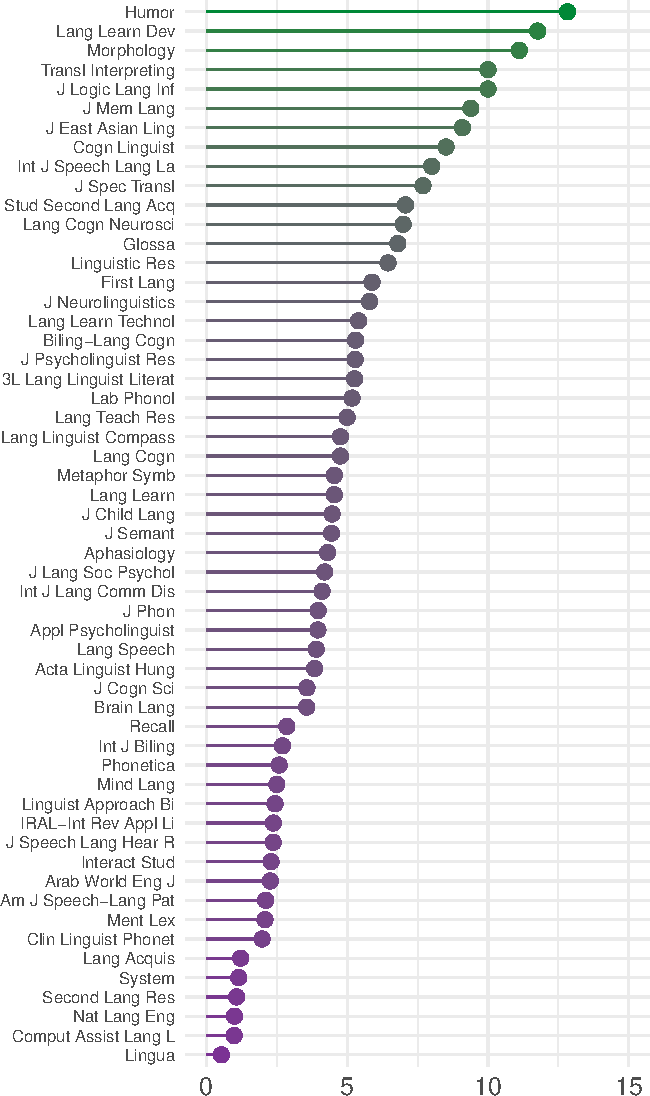
\includegraphics[width=1\linewidth]{ReplicationLing_files/figure-latex/topten_plot-1} \end{center}

Following preregistered protocol, we estimated the mention rate as
predicted relative to the following factors: journal impact factors
(continuous), open access (binary: open access journal or not), and
replication policies (binary: either explicitly encourage or not). We
used Bayesian parameter estimation based on generalized linear
regression models with a binomial link function. The model will be
fitted to the proportion of replication mentions per journal using the R
package brms (Bürkner, 2016). We used weakly informative normal priors
centered on 0 (sd = 2.5) for the intercept and Cauchy priors centered on
zero (scale = 2.5) for all population-level regression coefficients.
These priors are what is referred to as regularizing (Gelman et al.,
2008), i.e.~our prior assumption is agnostic as to whether the
predictors affect the dependent variable, thus making our model
conservative with regards to the predictors under investigation. Four
sampling chains with 2000 iterations each will be run for each model,
with a warm-up period of 1000 iterations. For relevant predictor levels
and contrasts between predictor levels, we will report the posterior
probability for the rate of replication mention. We summarize these
distributions by reporting the posterior mean and the 95\% credible
intervals (calculated as the highest posterior density interval).

The model estimates a replication mention rate of 0.03 {[}0.02, 0.04{]}
at a JIF of 0 and estimates a rather robust increase of the rate with
each unit of JIF (log odds = 0.39 {[}0.29, 0.49{]}). FigureX illustrates
this relationship.

However, further explorations indicate that JIF is highly correlated
with the number of experimental studies reported in a journal (Spearman
correlation = 0.4274344). This makes intuitively sense. Experimental
linguistic articles are often associated with psychology adjacent
fields, possibly attracting a broader audience and being cited more
widely. Given this correlation, it remains unclear if the term
"replicat*" is used more often in high impact journals or simply more
common in journals that generally publish more experimental studies.

\begin{center}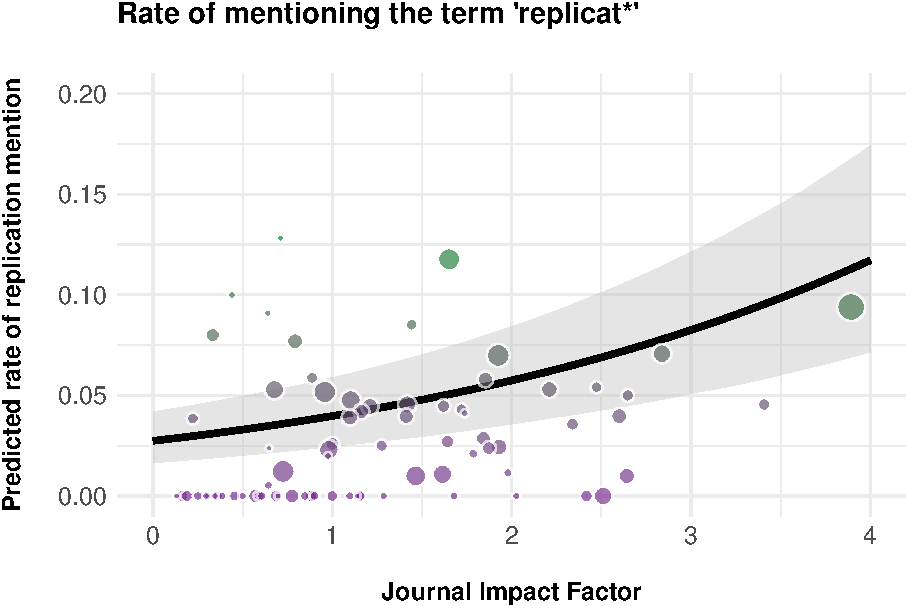
\includegraphics[width=1\linewidth]{ReplicationLing_files/figure-latex/plot_mention_jif-1} \end{center}

The model estimates the impact of whether the journal is open access or
not and whether replications are explicitly encouraged or not both as
positive, i.e.~more replication mentions in both open access and
explicitly encouraging journals, but the uncertainty around these
estimates is substantial (open access: 0.41 {[}-0.41, 1.14{]}; policy:
0.24 {[}-0.27, 0.72{]}). The large amount of uncertainty surrounding the
estimates is not surprising given the small number of journals that
explicitly encourage direct replications (2 out of 98), and the small
number of open access journals (11 out of 98).

\hypertarget{discussion}{%
\subsubsection{Discussion}\label{discussion}}

\begin{itemize}
\tightlist
\item
  too little replication attempts in experimental linguistics
\item
  journals guidelines generally don't encourage replication studies
\item
  \ldots{}
\end{itemize}

\hypertarget{detailed-analysis-types-and-contributing-factors}{%
\section{Detailed analysis: types and contributing
factors}\label{detailed-analysis-types-and-contributing-factors}}

The second part of the study aimed at obtaining a better understanding
of the underlying mechanisms of replication attempts published in the
field of experimental linguistics. Because the term ``replication'' is
commonly used in ambiguous ways, the articles that contained the search
term ``replicat*'' required further analysis to determine whether the
articles in question indeed reported a replication study or used the
term in a different way.

We were interested in which kinds of replication studies are published
and which factors contribute to their publication. We aimed at
investigating what types of replication studies are prevalent in the
field. We were further interested in the relationship of direct
replications and whether the paper was published as open access or not,
the number of citations of the initial study and the years between
publication of the initial study and the replication attempt.

\hypertarget{material-and-methods-1}{%
\subsubsection{Material and methods}\label{material-and-methods-1}}

The material and methods have been preregistered on Open Science
Framework and can be inspected \href{https://osf.io/9ceas/}{here:
https://osf.io/9ceas/}.

From the superset of 100 journals obtained above, the first 20 journals
(i.e.~those journals with the highest proportion of experimental
studies) were selected for a more detailed analysis while excluding
journals for which less than 2 hits (TS=(replicat*)) could be obtained
(see \href{https://osf.io/f3yp8/}{here} for a list of article counts per
journal: https://osf.io/f3yp8/). Because of the skewed distribution of
our sample (114 hits for Journal of Memory and Language, and less than
40 for all other journals), we randomly selected 50 out of the 114
articles for the Journal of Memory and Language to achieve a more
balanced distribution of papers across journals (see
\href{https://osf.io/6vfpe/}{here} for details). The sampling procedure
above resulted in 210 possible self-labeled replication studies.

In a first step, we identified whether the article in question indeed
presented a replication study or not. The relevant parts of the papers
were title and abstract of the paper, sentences around occurrences of
the search term ``replicat'' as well as the paragraph before the Methods
section and the first paragraph of the Discussion section (following the
procedure specified by Makel et al. (2016)). If the authors explicitly
claimed that (one of) their research aim(s) was to replicate or
reproduce findings or methods of an initial study, this article was
treated as a replication. It then qualified for further analysis after
the coding scheme that can be viewed \href{https://osf.io/ct2xj/}{here}:
https://osf.io/ct2xj/.

When extracting number and types of changes made to the initial study,
we assumed that the authors of a replication study did not make any
drastic changes \emph{without} reporting them. The replication studies
were classified according to three types: direct replication (0
changes), partial replication (1 change) and conceptual replication (2
or more changes), following Marsden et al. (2018). We noted the nature
of the change as one of the following categories (yes/no): experimental
paradigm, sample, materials/experimental set-up, dependent variable,
independent variable, and control. We also noted the language under
investigation. The information on whether the article was published open
access as well as citation counts and years of publication for both
studies were obtained from Web of Science. An author overlap was
attested when one of the authors was a (co-)author on both articles.

\hypertarget{results-1}{%
\subsubsection{Results}\label{results-1}}

Out of the 210 articles in the subsample, 117 were self-claimed
replications according to our criteria. The remaining 93 mentions were
xxx. Out of these replication studies, we categorized 66 as conceptual,
42 as partial, and only 8 as direct replications which amounts to
6.83760683760684\% of all coded cases.

Looking closer at direct replications, 3 studies were independent
studies, i.e.~there was no overlap between authors of the original study
and the replication study. Out of these independent direct replication
studies, 5 were self-labeled as successful replications. In other words,
our sample did not include a single independent failed replication
attempt.

To paint a more general picture by including all types of replications,
31.6239316239316\% studies are replications within the same multi-study
paper. One central aspect of linguistic research is the testing the
generalizability of experimental claims across different target
languages, however, as it turns out only a minority of replications
targeted a different language than the initial study
(15.3846153846154\%). The majority of replication efforts were conducted
within the same language as the initial study.

Comparing original study to replication study, 0\% of replications are
published in the same journal as the initial study. The median number of
years between an initial and a replication study is 7. Initial studies
were on average 41.1 times cited before a replication was published
which amounts to a average mean citation rate of 5.9.

\begin{verbatim}
## type_replication
## conceptual     direct    partial 
##       0.44       0.09       0.47
\end{verbatim}

\begin{verbatim}
##                 auth_overlap
## type_replication    0    1
##       conceptual 0.18 0.26
##       direct     0.06 0.03
##       partial    0.24 0.24
\end{verbatim}

\begin{verbatim}
## [1] 0.04
\end{verbatim}

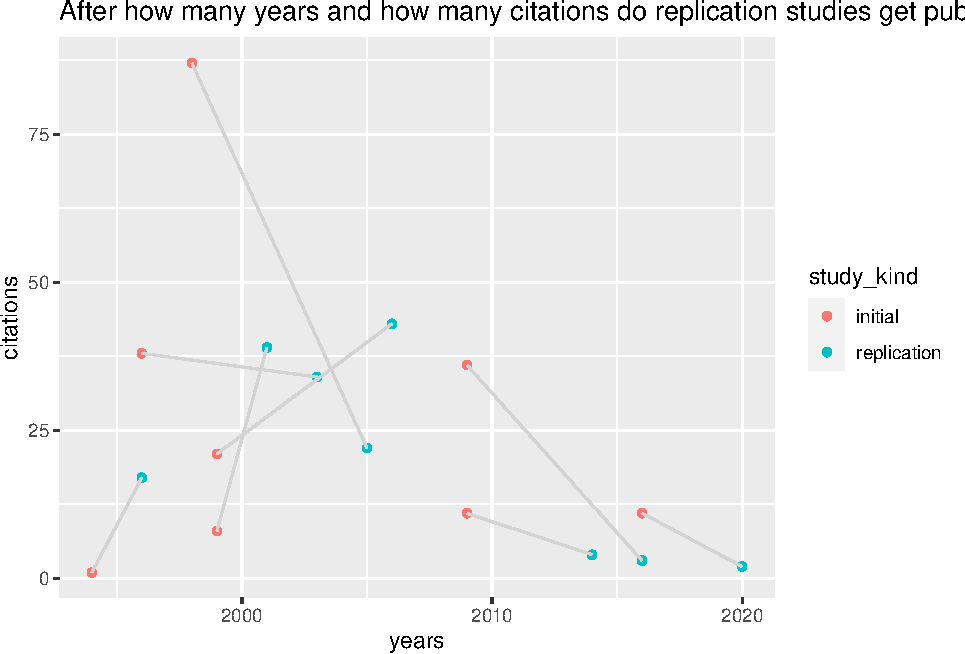
\includegraphics{ReplicationLing_files/figure-latex/plot cit and years direct-1.pdf}

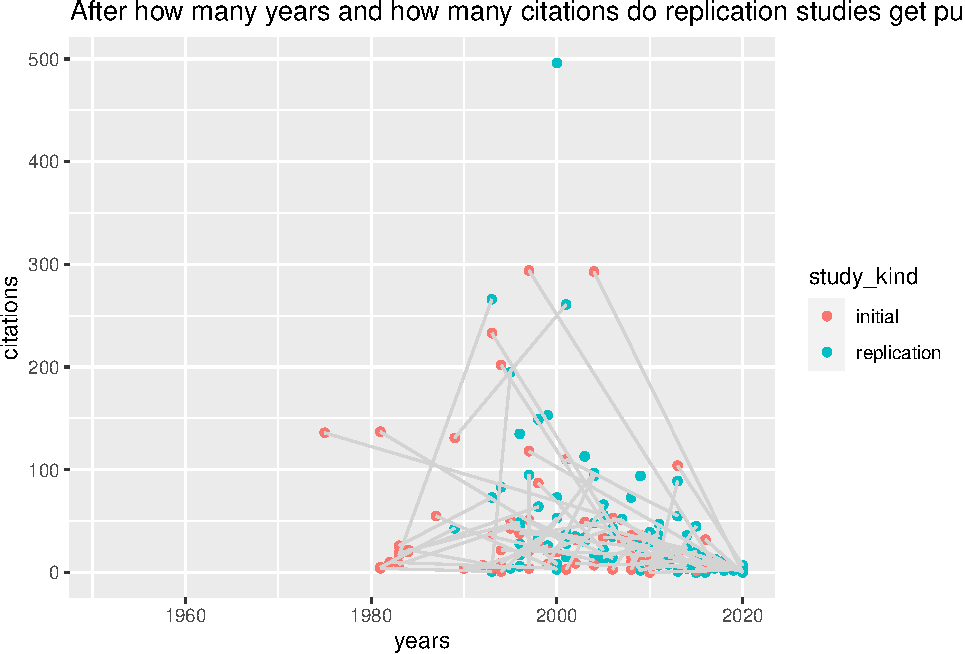
\includegraphics{ReplicationLing_files/figure-latex/plot cit and years all-1.pdf}

\hypertarget{discussion-1}{%
\subsubsection{Discussion}\label{discussion-1}}

\hypertarget{general-discussion}{%
\section{General discussion}\label{general-discussion}}

\begin{itemize}
\tightlist
\item
  compare rate of replication mention to previous studies in different
  fields --\textgreater{} broader picture
\end{itemize}

\hypertarget{caveats}{%
\subsubsection{Caveats}\label{caveats}}

This procedure is necessarily only a rough proxy of relevant
experimental linguistic articles published in the field and several
articles might thus have been overlooked and not been included in the
analysis.

\hypertarget{appendices}{%
\section{Appendices}\label{appendices}}

identified as A, B, etc.

\hypertarget{references}{%
\section*{References}\label{references}}
\addcontentsline{toc}{section}{References}

\hypertarget{refs}{}
\begin{CSLReferences}{1}{0}
\leavevmode\hypertarget{ref-burkner_brms_2016}{}%
Bürkner, P.-C., 2016. Brms: {An} {R} package for {Bayesian} multilevel
models using {Stan}. Journal of Statistical Software 80, 1--28.

\leavevmode\hypertarget{ref-camerer_economics_2016}{}%
Camerer, C.F., Dreber, A., Forsell, E., Ho, T.-H., Huber, J.,
Johannesson, M., Kirchler, M., Almenberg, J., Altmejd, A., Chan, T.,
Heikensten, E., Holzmeister, F., Imai, T., Isaksson, S., Nave, G.,
Pfeiffer, T., Razen, M., Wu, H., 2016. Evaluating replicability of
laboratory experiments in economics. Science 351, 1433--1436.
doi:\href{https://doi.org/10.1126/science.aaf0918}{10.1126/science.aaf0918}

\leavevmode\hypertarget{ref-camerer_socscience_2018}{}%
Camerer, C.F., Dreber, A., Holzmeister, F., Ho, T.-H., Huber, J.,
Johanesson, M., Kirchler, M., Nave, G., Nosek, B.A., Pfeiffer, T.,
Altmejd, A., Buttrick, N., Chan, T., Chen, Y., Forsell, E., Gampa, A.,
Heikensten, E., Hummer, L., Imai, T., Isaksson, S., Manfredi, D., Rose,
J., Wagenmakers, E.-J., Wu, H., 2018. Evaluating the replicability of
social science experiments in nature and science between 2010 and 2015.
Nature 2, 637--644.
doi:\href{https://doi.org/10.1038/s41562-018-0399-z}{10.1038/s41562-018-0399-z}

\leavevmode\hypertarget{ref-chen_chinese_2007}{}%
Chen, J.-Y., 2007. Do {Chinese} and {English} speakers think about time
differently? {Failure} of replicating {Boroditsky} (2001). Cognition
104, 427--436.

\leavevmode\hypertarget{ref-gelman_weakly_2008}{}%
Gelman, A., Jakulin, A., Pittau, M.G., Su, Y.-S., others, 2008. A weakly
informative default prior distribution for logistic and other regression
models. The Annals of Applied Statistics 2, 1360--1383.

\leavevmode\hypertarget{ref-makel2014facts}{}%
Makel, M.C., Plucker, J.A., 2014. Facts are more important than novelty:
Replication in the education sciences. Educational Researcher 43,
304--316.

\leavevmode\hypertarget{ref-makel_replications_2016}{}%
Makel, M.C., Plucker, J.A., Freeman, J., Lombardi, A., Simonsen, B.,
Coyne, M., 2016. Replication of special education research: Necessary
but far too rare. Remedial and Special Education 37, 205--212.

\leavevmode\hypertarget{ref-makel_replications_2012}{}%
Makel, M.C., Plucker, J.A., Hegarty, B., 2012. Replications in
psychology research: {How} often do they really occur? Perspectives on
Psychological Science 7, 537--542.

\leavevmode\hypertarget{ref-marsden_replication_2018}{}%
Marsden, E., Morgan‐Short, K., Thompson, S., Abugaber, D., 2018.
Replication in {Second} {Language} {Research}: {Narrative} and
{Systematic} {Reviews} and {Recommendations} for the {Field}. Language
Learning 68, 321--391. doi:\href{https://doi.org/gc3h3b}{gc3h3b}

\leavevmode\hypertarget{ref-martinclarke_policies_2017}{}%
Martin, G.N., Clarke, R.M., 2017. Are psychology journals
anti-replication? A snapshot of editorial practices. Frontiers in
Psychology 8.
doi:\href{https://doi.org/10.3389/fpsyg.2017.00523}{10.3389/fpsyg.2017.00523}

\leavevmode\hypertarget{ref-nieuwland_large-scale_2018}{}%
Nieuwland, M.S., Politzer-Ahles, S., Heyselaar, E., Segaert, K., Darley,
E., Kazanina, N., Zu Wolfsthurn, S.V.G., Bartolozzi, F., Kogan, V., Ito,
A., Mézière, D., Barr, D.J., Rousselet, G.A., Ferguson, H.J.,
Bush-Moreno, S., Fu, X., Tuomainen, J., Kulakova, E., Husband, M.E.,
Donaldson, D.I., Kohút, Z., Rueschemeyer, S.-A., Huettig, F., 2018.
Large-scale replication study reveals a limit on probabilistic
prediction in language comprehension. eLife 7, e33468.
doi:\href{https://doi.org/10.7554/eLife.33468.001}{10.7554/eLife.33468.001}

\leavevmode\hypertarget{ref-open_science_collaboration_estimating_2015}{}%
Open Science Collaboration, 2015. Estimating the reproducibility of
psychological science. Science 349.
doi:\href{https://doi.org/10.1126/science.aac4716}{10.1126/science.aac4716}

\leavevmode\hypertarget{ref-papesh_just_2015}{}%
Papesh, M.H., 2015. Just out of reach: {On} the reliability of the
action-sentence compatibility effect. Journal of Experimental
Psychology: General 144, e116--e141.
doi:\href{https://doi.org/10.1037/xge0000125}{10.1037/xge0000125}

\leavevmode\hypertarget{ref-roettger2019toward}{}%
Roettger, T.B., Baer-Henney, D., 2019. Toward a replication culture:
Speech production research in the classroom. Phonological Data and
Analysis 1, 1--23.

\leavevmode\hypertarget{ref-stack_failure_2018}{}%
Stack, C.M.H., James, A.N., Watson, D.G., 2018. A failure to replicate
rapid syntactic adaptation in comprehension. Memory \& Cognition 46,
864--877.
doi:\href{https://doi.org/10.3758/s13421-018-0808-6}{10.3758/s13421-018-0808-6}

\leavevmode\hypertarget{ref-westbury_implicit_2018}{}%
Westbury, C., 2018. Implicit sound symbolism effect in lexical access,
revisited: {A} requiem for the interference task paradigm. Journal of
Articles in Support of the Null Hypothesis 15, 1--12.

\end{CSLReferences}


\end{document}
